\documentclass[10pt,a4paper]{article}
\usepackage[utf8]{inputenc}
\usepackage{amsmath}
\usepackage{amsfonts}
\usepackage{amssymb}
\usepackage{amsthm}
\usepackage{graphicx}
\usepackage[russian]{babel}
\newcommand{\Pb}{\mathbb{Pb}}
\author{Антон Бакутеев}
\title{Домашнее задание на 19 апреля}
\newtheorem{task}{Задание}
\begin{document}
	\maketitle
	\begin{task}
		Доказать, что сумма квадратов двух независимых случайных величин, равномерно распределённых на отрезке $[-1, +1]$, будет равномерно распределена на первой половине промежутка $[0, 2]$.
	\end{task}
	\begin{proof}
		Рассмотрим случайные величины $ \xi_1, \xi_2 \sim U[-1, 1] $. Тогда случайную величину $ z = \xi_1^2 + \xi_2^2 $ можно представить на координатной плоскости. Ее распределение соответствует площади круга на Рис.~\ref{fig:circle}.
		\[ \Pb(z < x)  = \Pb\left(\frac{\text{площадь круга с радиусом } \sqrt{x}}{\text{площадь квадрата}}\right) = \frac{\pi x}{4}, \hspace{5pt} \forall x\in[0, 1]\]
		\begin{figure}[h]
			\centering
			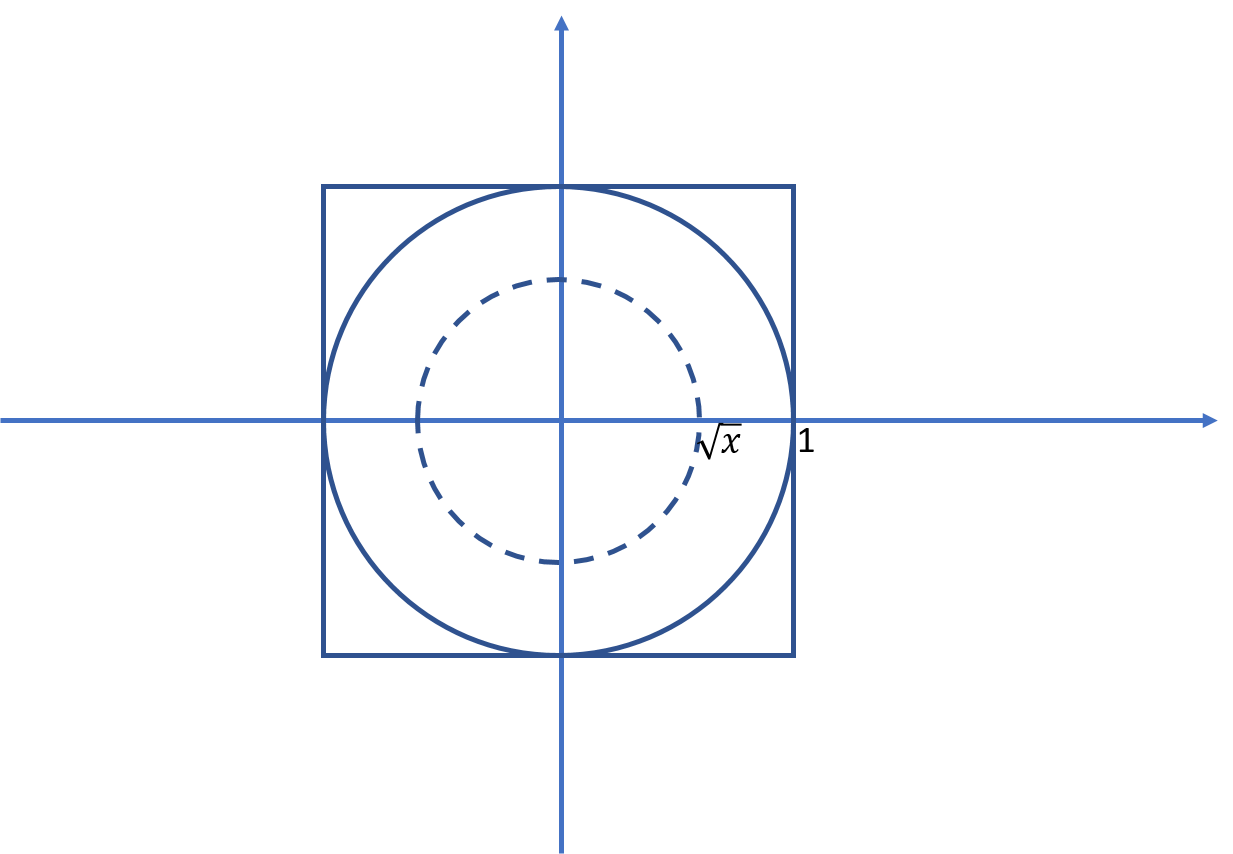
\includegraphics[width=0.7\linewidth]{circle}
			\caption{Геометрическое представление}
			\label{fig:circle}
		\end{figure}
		
		Следовательно, случайная величина $  \xi_1^2 + \xi_2^2 $ равномерно распределена на первой половине промежутка $[0, 2]$, так как вероятности попадания в каждую из точек этой половины равны.
	\end{proof}
\end{document}